A continuación se procede a explicar la construcción del brazo robotico. Para ello, se emplearán los diseños 3D y ciertas imágenes del brazo real en sus etapas de construcción.

La razón de no explicar el proceso integro con imágenes reales del brazo es debido a que no hay suficientes documentos gráficos para ejemplificar el proceso completo y ciertas etapas de la construcción quedarían sin poder ser documentadas.

\begin{figure}[H]
    \centering 
    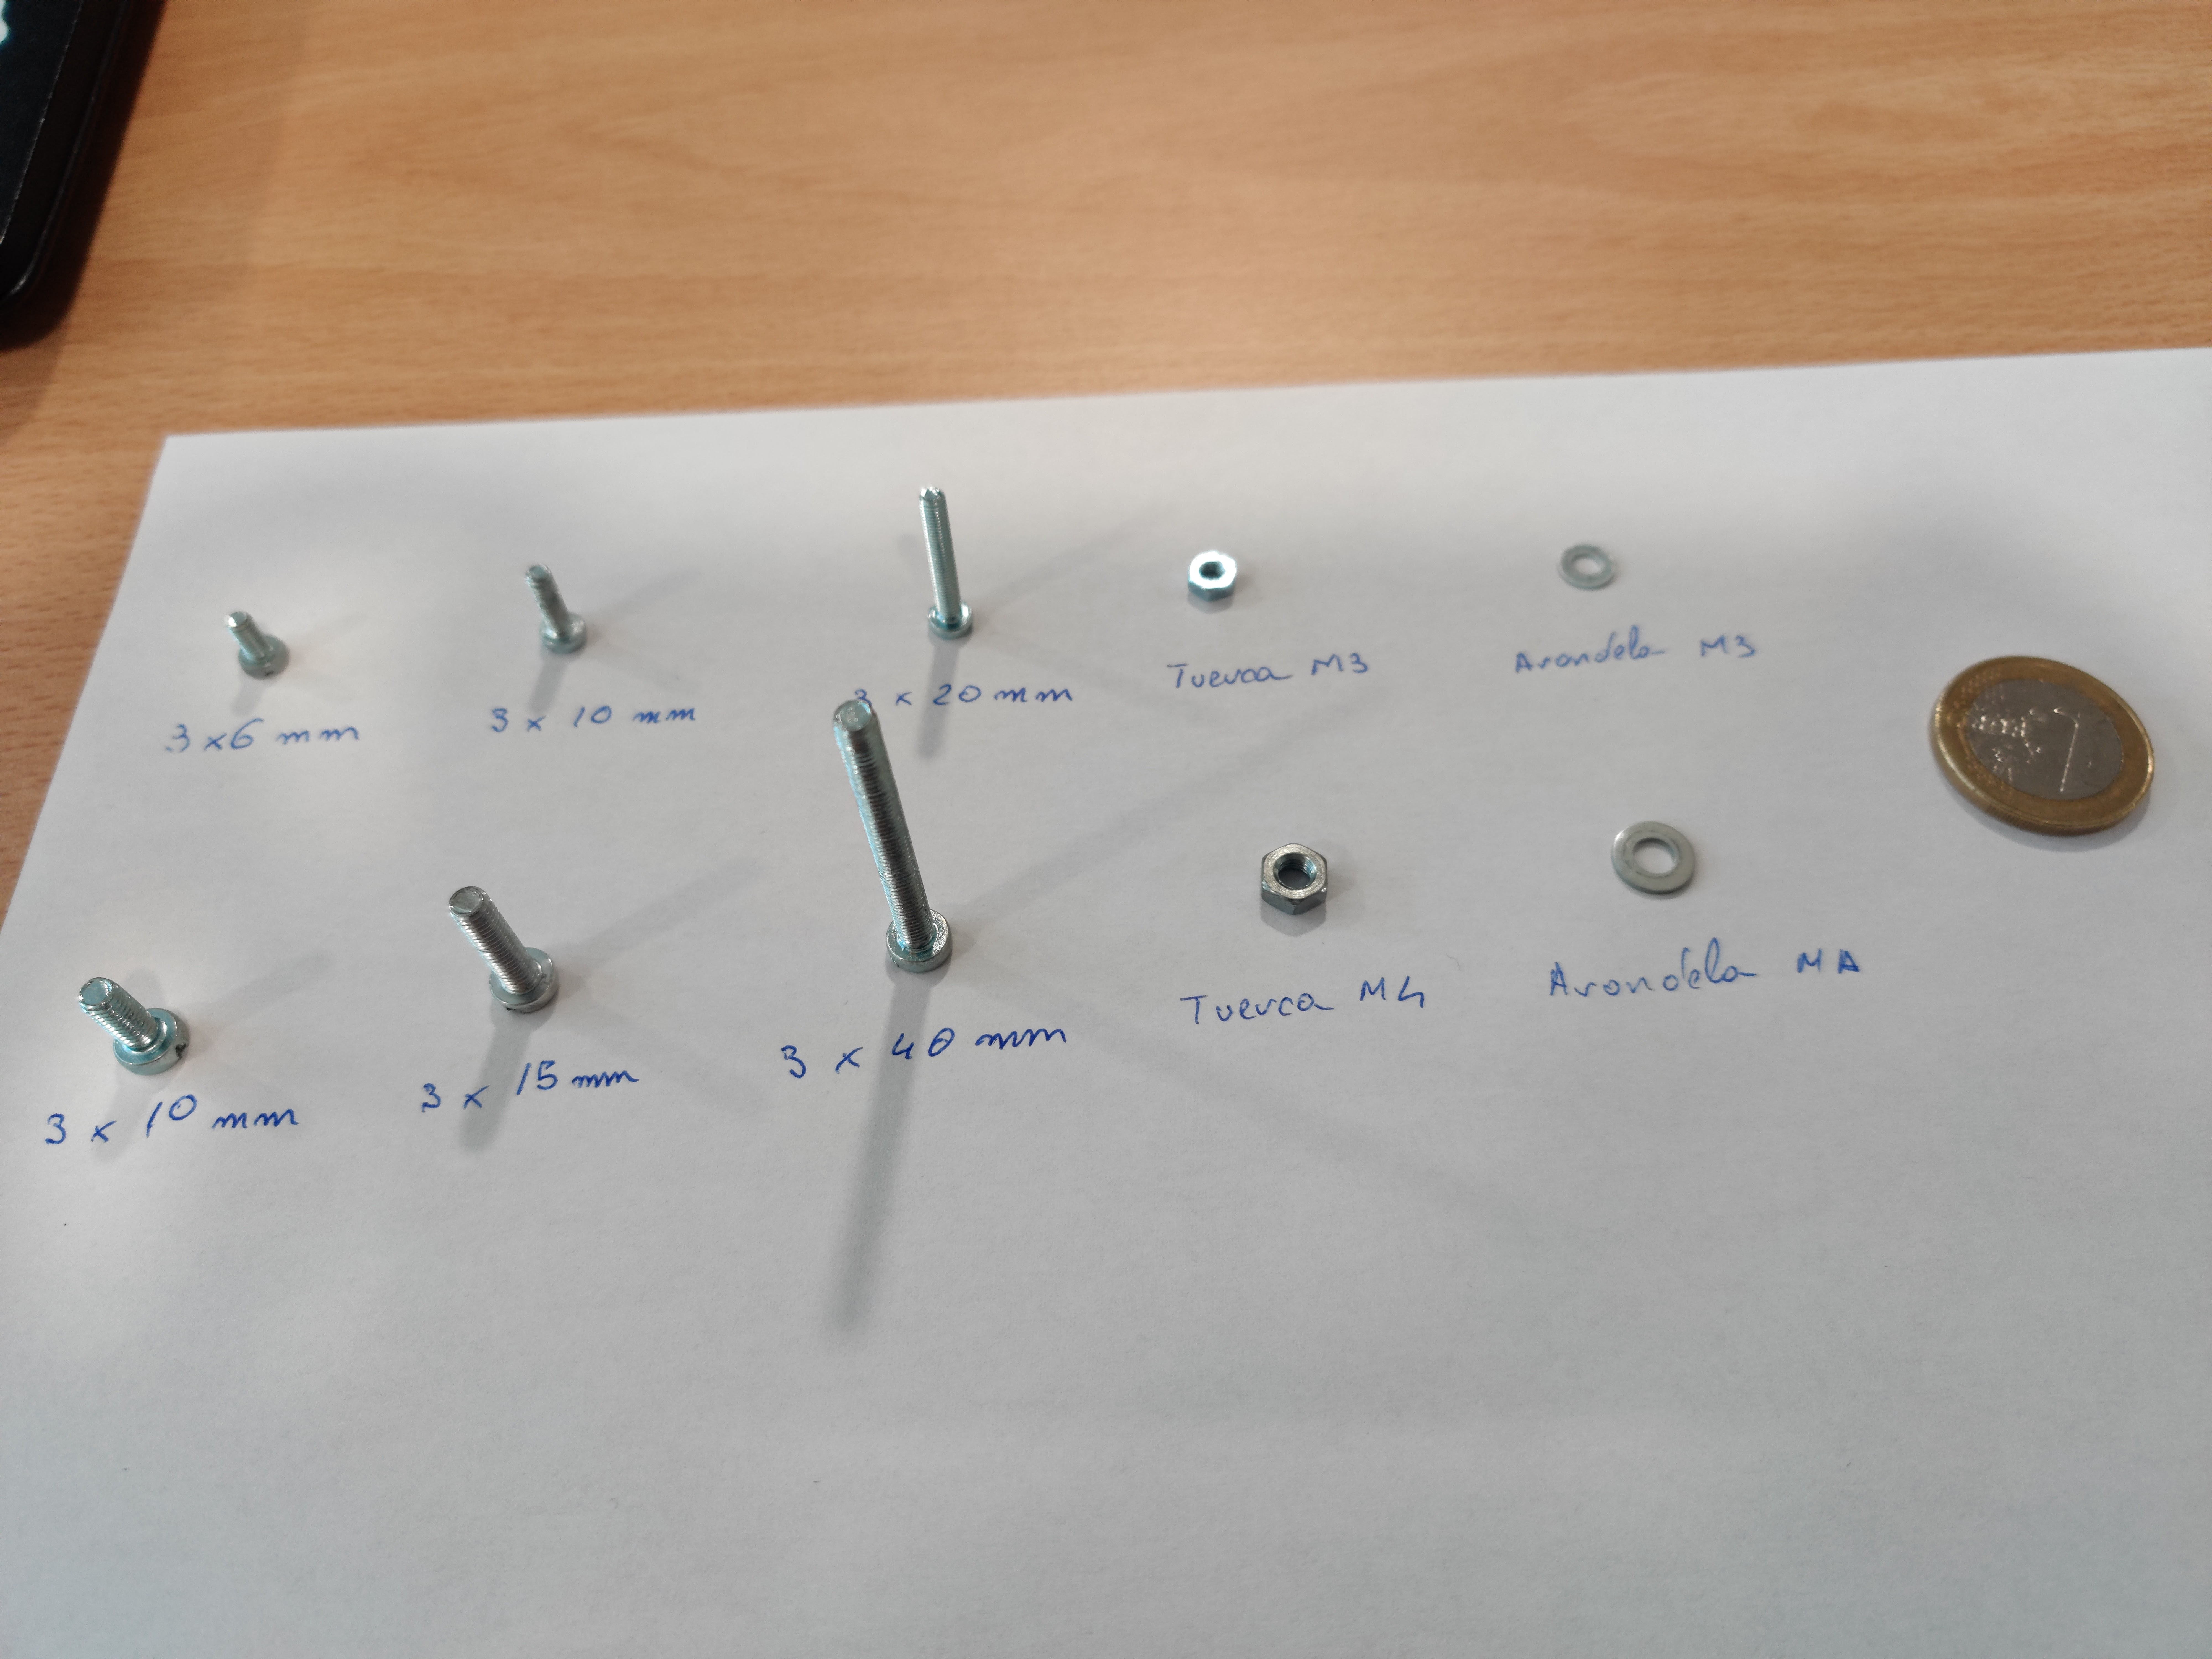
\includegraphics[width=1\linewidth]{pictures/ElementosMecanicosExternos.jpg}
    \caption{Elementos mecánicos externos}
    \label{fig:elementos_mecanicos_externos}
\end{figure}

En la figura \ref{fig:elementos_mecanicos_externos} se pueden observar los distintos tornillos, tuercas y arandelas que se emplearan a lo largo de la construcción del brazo. Esta imagen puede servir como referencia para tener una imagen real de los diferentes elementos externos que se nombrarán a lo largo de la explicación.

\begin{figure}[H]
    \centering 
    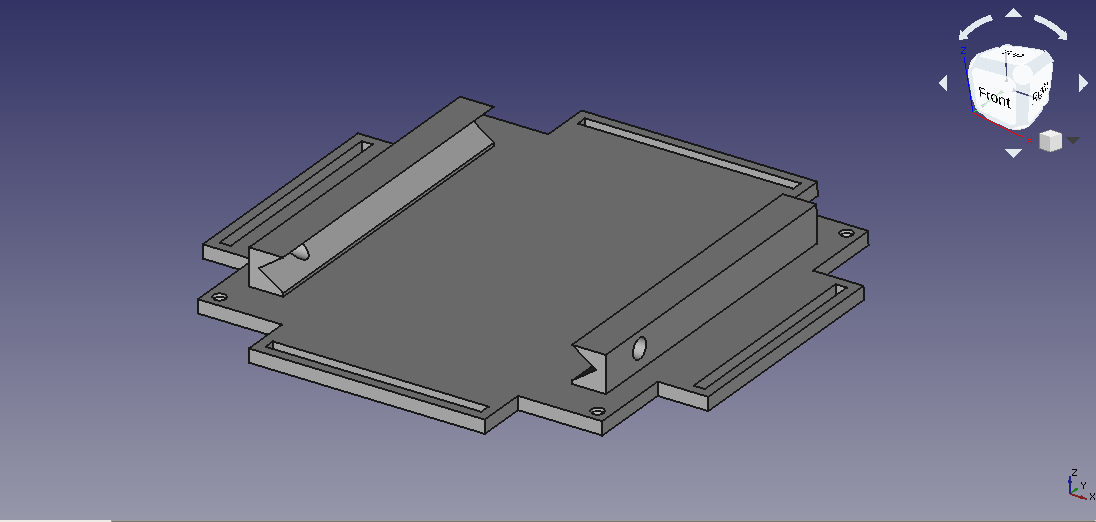
\includegraphics[width=1\linewidth]{pictures/BaseDelBrazoRobotico.png}
    \caption{Base de la caja del brazo robótico}
    \label{fig:base_caja_brazo_robotico}
\end{figure}

\begin{figure}[H]
    \centering 
    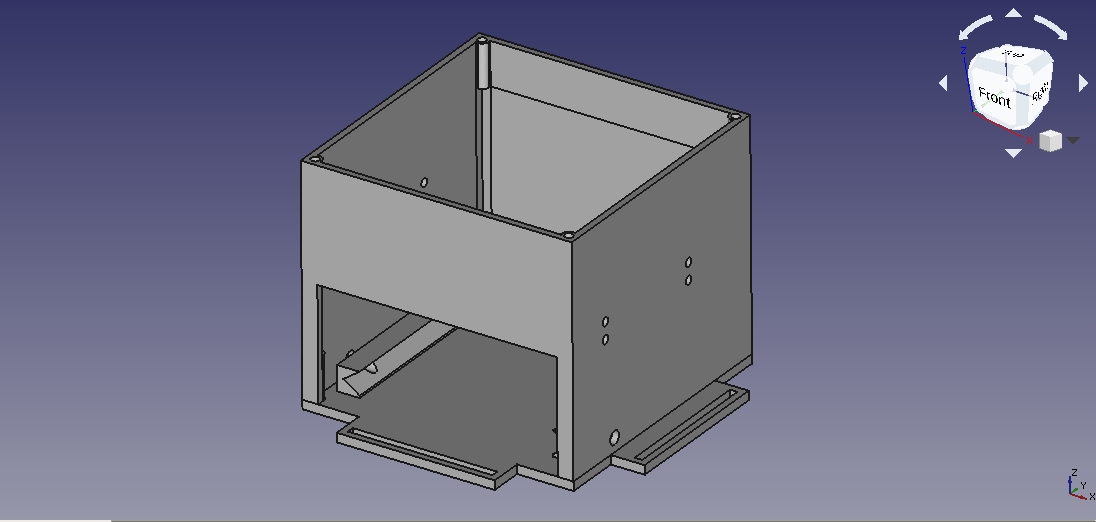
\includegraphics[width=1\linewidth]{pictures/BaseYParedes.png}
    \caption{Base y paredes de la caja del brazo robótico}
    \label{fig:base_paredes_caja_brazo_robotico}
\end{figure}

\begin{figure}[H]
    \centering 
    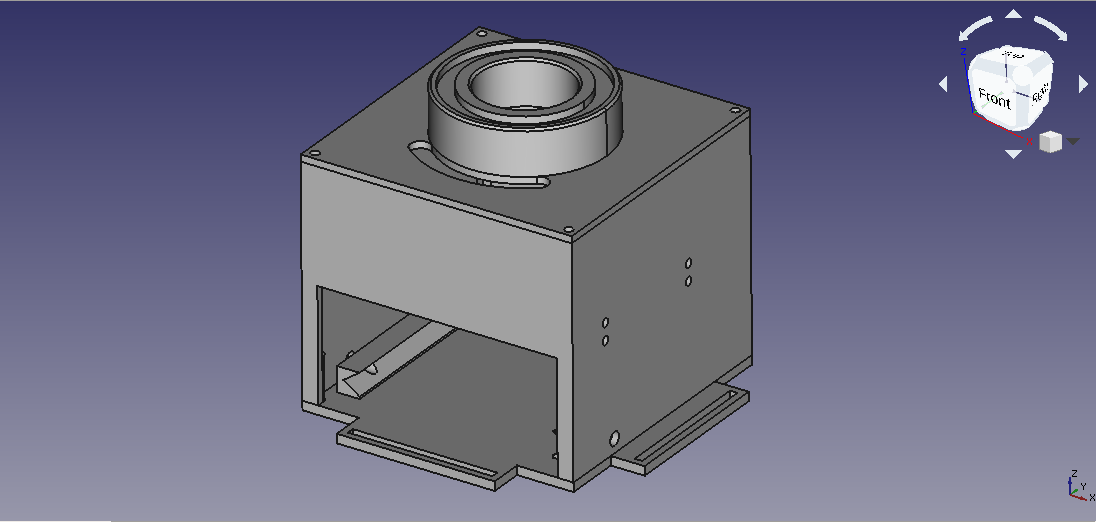
\includegraphics[width=1\linewidth]{pictures/CajaCompleta.png}
    \caption{Caja completa del brazo robótico}
    \label{fig:caja_completa_brazo_robotico}
\end{figure}

Como observamos en las figuras \ref{fig:base_caja_brazo_robotico}, \ref{fig:base_paredes_caja_brazo_robotico} y \ref{fig:caja_completa_brazo_robotico} la caja esta compuesta por 3 piezas y estas se ensamblan verticalmente una encima de otra mediante tornillo de 4x15 cm.
Cabe destacar que esta parte de la estructura es inmóvil y sirve como soporte para la parte móvil.

\begin{figure}[H]
    \centering 
    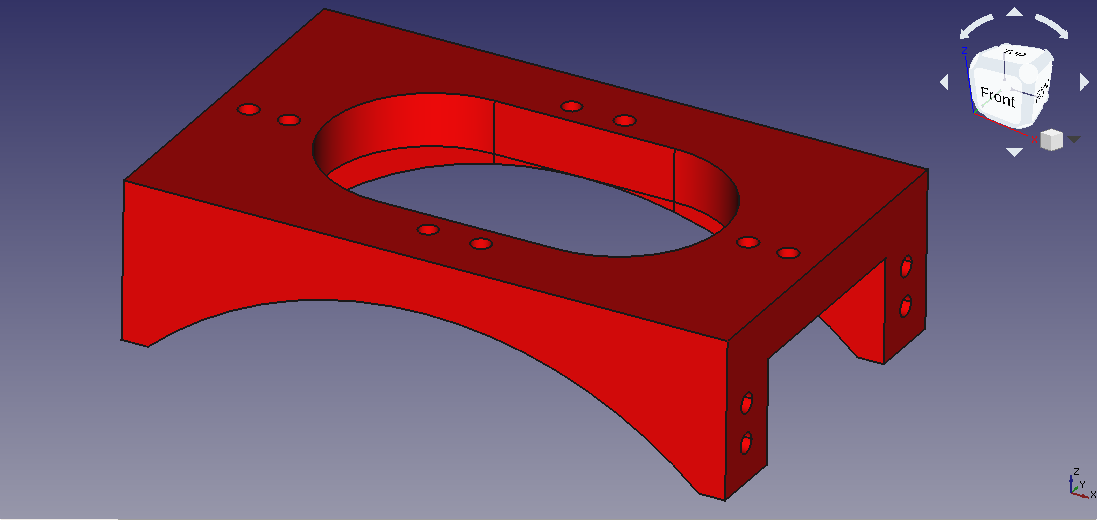
\includegraphics[width=1\linewidth]{pictures/MotorHold.png}
    \caption{Sujeción del motor de la base}
    \label{fig:sujección_motor_base}
\end{figure}

\begin{figure}[H]
    \centering 
    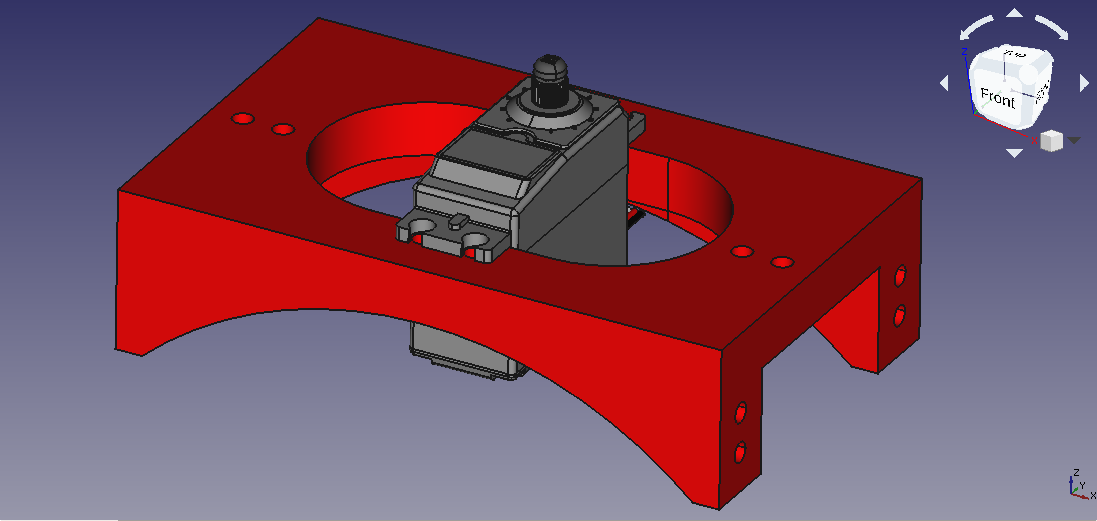
\includegraphics[width=1\linewidth]{pictures/MotorHoldYMotor.png}
    \caption{Motor de la base ensamblado en su soporte}
    \label{fig:motor_ensamblado_soporte}
\end{figure}

\begin{figure}[H]
    \centering 
    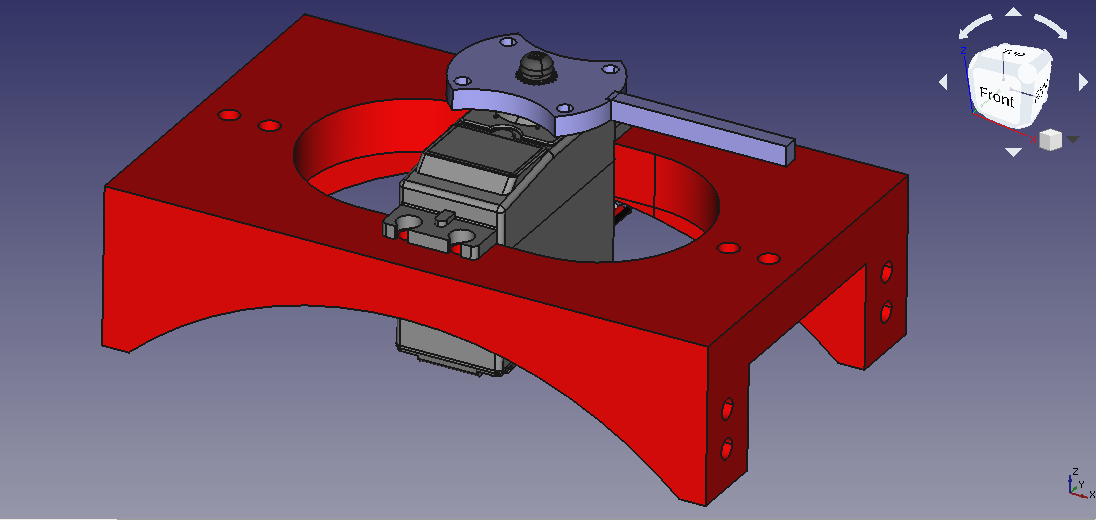
\includegraphics[width=1\linewidth]{pictures/MotorMasPrimeraPieza.png}
    \caption{Primera pieza del sistema de transmisión del movimiento}
    \label{fig:primera_pieza_sistema_transmision}
\end{figure}

\begin{figure}[H]
    \centering 
    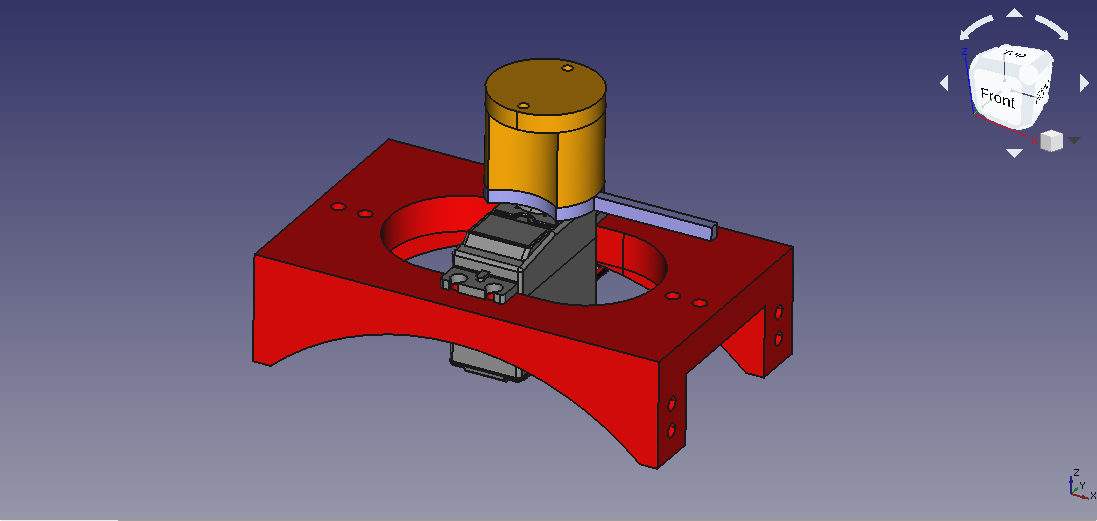
\includegraphics[width=1\linewidth]{pictures/MotorMasSegundaPieza.png}
    \caption{Segunda pieza del sistema de transmisión del movimiento}
    \label{fig:segunda_pieza_sistema_transmision}
\end{figure}

\begin{figure}[H]
    \centering 
    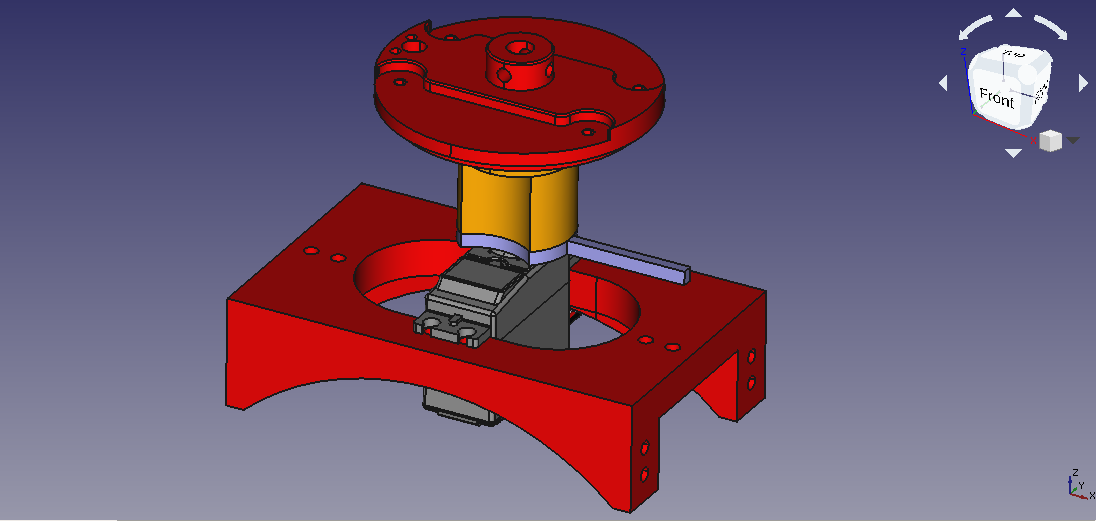
\includegraphics[width=1\linewidth]{pictures/MotorMasTerceraPieza.png}
    \caption{Tercera pieza del sistema de transmisión del movimiento}
    \label{fig:tercera_pieza_sistema_transmision}
\end{figure}

\begin{figure}[H]
    \centering 
    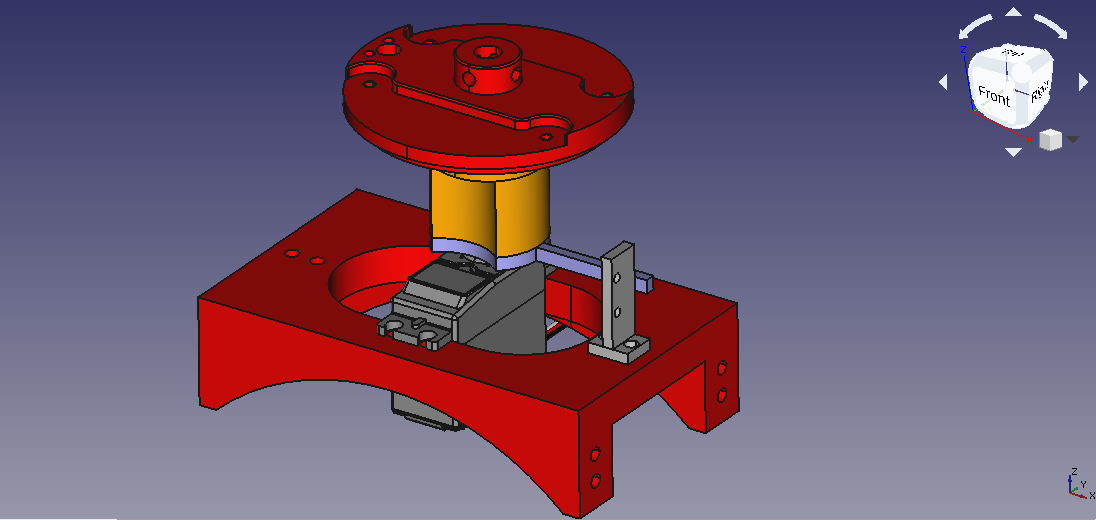
\includegraphics[width=1\linewidth]{pictures/FinalDeCarrera.png}
    \caption{Cadena de transmisión final con soporte para fin de carrera}
    \label{fig:sistema_transmision_fin_carrera}
\end{figure}

En las figuras \ref{fig:sujección_motor_base}, \ref{fig:motor_ensamblado_soporte}, \ref{fig:primera_pieza_sistema_transmision},
\ref{fig:segunda_pieza_sistema_transmision},
\ref{fig:tercera_pieza_sistema_transmision} y \ref{fig:sistema_transmision_fin_carrera} se observan los componentes que servirán para transmitir el movimiento desde el motor a la base giratoria donde ira ensamblado el brazo robótico. Para asegurar el soporte a las paredes y posteriormente el motor al soporte se han empleado tornillos de 4x15 mm. Para los componentes que servirán para transmitir el movimiento, se han empleado tornillos de 3x10 mm debido a que las piezas son mas pequeñas y es necesario que los tornillos ocupen menos espacio.

\begin{figure}[H]
    \centering 
    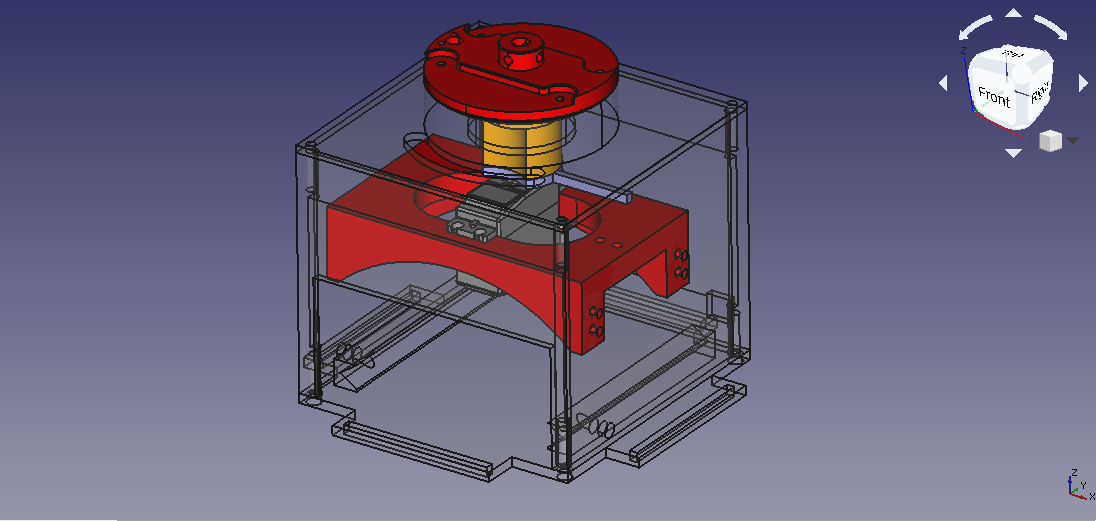
\includegraphics[width=1\linewidth]{pictures/CajaConPiezasInternas.png}
    \caption{Interior de la caja}
    \label{fig:interior_caja_sujeccion}
\end{figure}

Sobre la base giratoria superior será montado ahora el sistema de motores que se encargará de mover el brazo en el eje vertical.

\begin{figure}[H]
    \centering 
    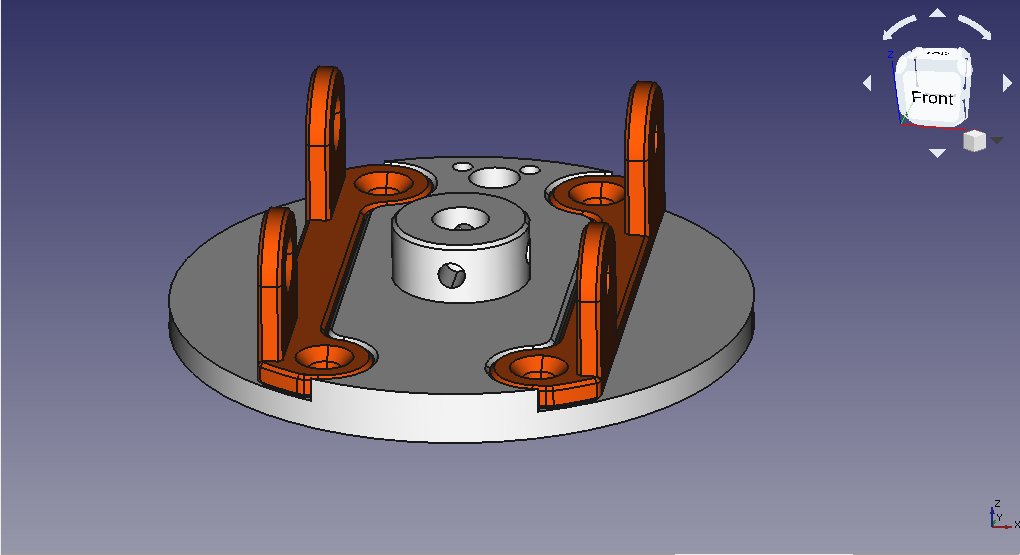
\includegraphics[width=1\linewidth]{pictures/BaseRotatoriaConPletinas.png}
    \caption{Base rotatoria con pletinas}
    \label{fig:base_rotatoria_pletinas}
\end{figure}

En la figura \ref{fig:base_rotatoria_pletinas} se observa que las pletinas que sujetaran los motores a la base encajan en las hendiduras que existen en la base rotatoria. Estas pletinas son aseguradas a la base giratoria mediante tornillos 3x6 mm.

\begin{figure}[H]
    \centering 
    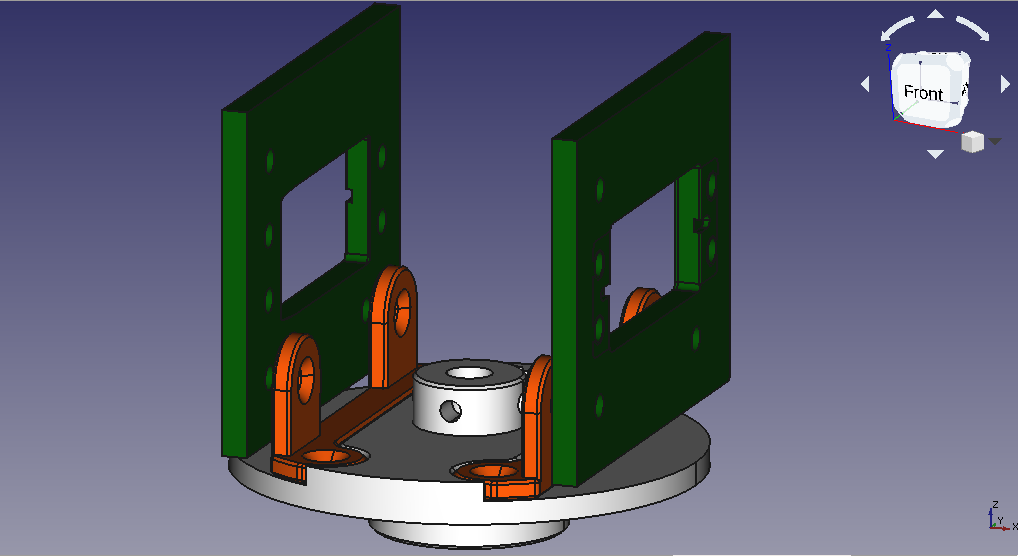
\includegraphics[width=1\linewidth]{pictures/BaseRotatoriaConPletinasYSoporte.png}
    \caption{Soporte para los motores laterales}
    \label{fig:soporte_motores_laterales}
\end{figure}

A continuación los soportes de los motores son añadidos a las pletinas y son asegurados a estas mediante tornillos de 4x15 mm con tuerca y arandela.
Entre la pletina y el soporte se puede observar una pequeña distancia, la cual se debe a un separador que existe en la construcción real pero que no aparece en el diseño 3D.

\begin{figure}[H]
    \centering 
    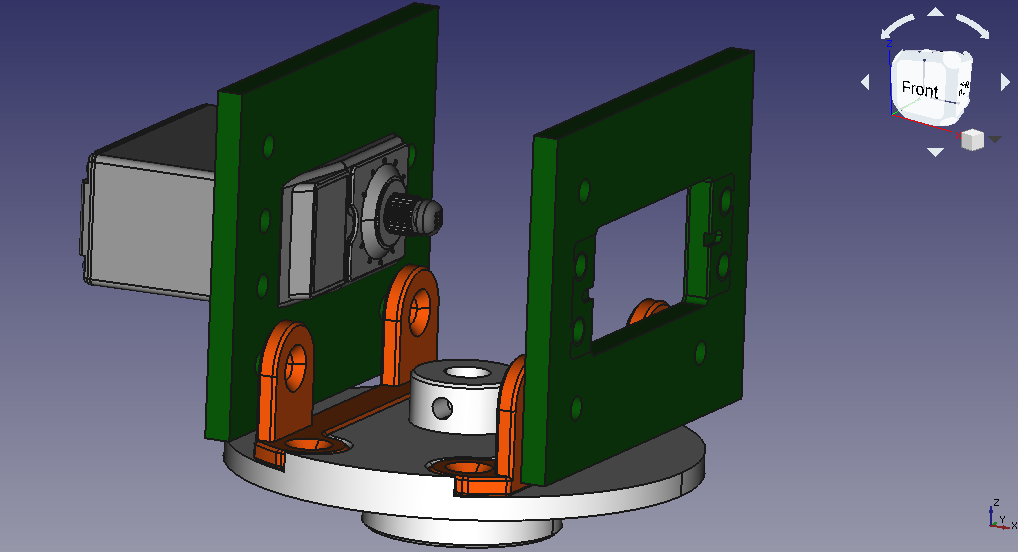
\includegraphics[width=1\linewidth]{pictures/BaseRotatoriaConUnMotor.png}
    \caption{Se añade uno de los motores}
    \label{fig:un_motor_añadido}
\end{figure}

Finalmente uno de los motores es añadidos a su soportes y es asegurado a este mediante tornillos de 4x10 mm con tuerca.

Por otro lado, es ensamblada la parte superior del del brazo según se indica a continuación.

\begin{figure}[H]
    \centering 
    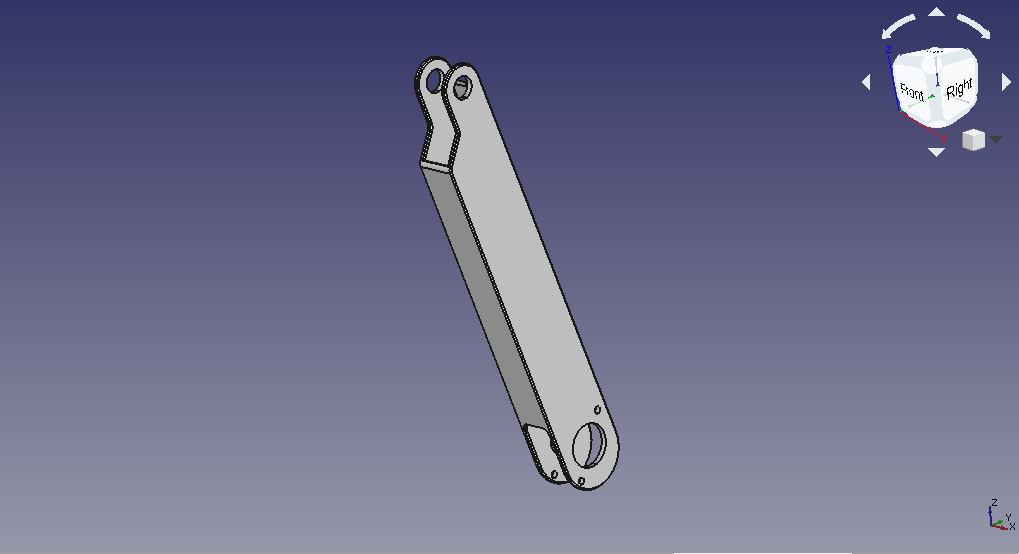
\includegraphics[width=1\linewidth]{pictures/SegmentoCentralBrazo.png}
    \caption{Segmento central del brazo robótico}
    \label{fig:segmento_central_brazo}
\end{figure}

\begin{figure}[H]
    \centering 
    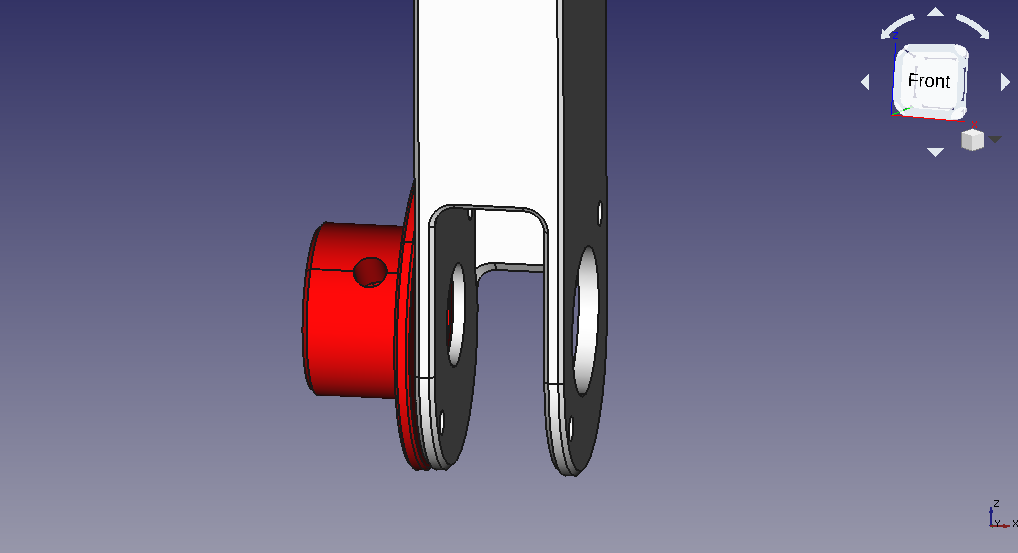
\includegraphics[width=1\linewidth]{pictures/SoporteMotorIzquierdo.png}
    \caption{Pieza izquierda de la cadena de movimiento vertical}
    \label{fig:pieza_izquierda_brazo}
\end{figure}

En las figuras \ref{fig:segmento_central_brazo} y \ref{fig:pieza_izquierda_brazo} se observa el montaje de la primera pieza de la cadena de movimiento vertical sobre el segmento central del brazo. Para asegurar la pieza al brazo se emplean tornillos 3x6 mm .

\begin{figure}[H]
    \centering 
    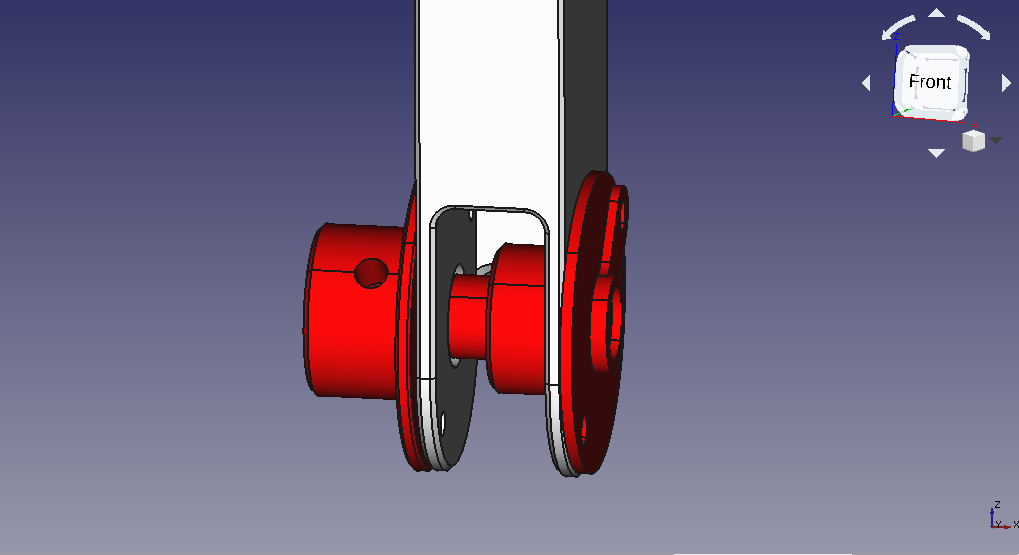
\includegraphics[width=1\linewidth]{pictures/SoporteMotorCentral.png}
    \caption{Pieza central de la cadena de movimiento vertical}
    \label{fig:pieza_central_brazo}
\end{figure}

En la figura \ref{fig:pieza_central_brazo} se monta la pieza central empleando los mismos tornillos de tamaño 3x6 mm.

\begin{figure}[H]
    \centering 
    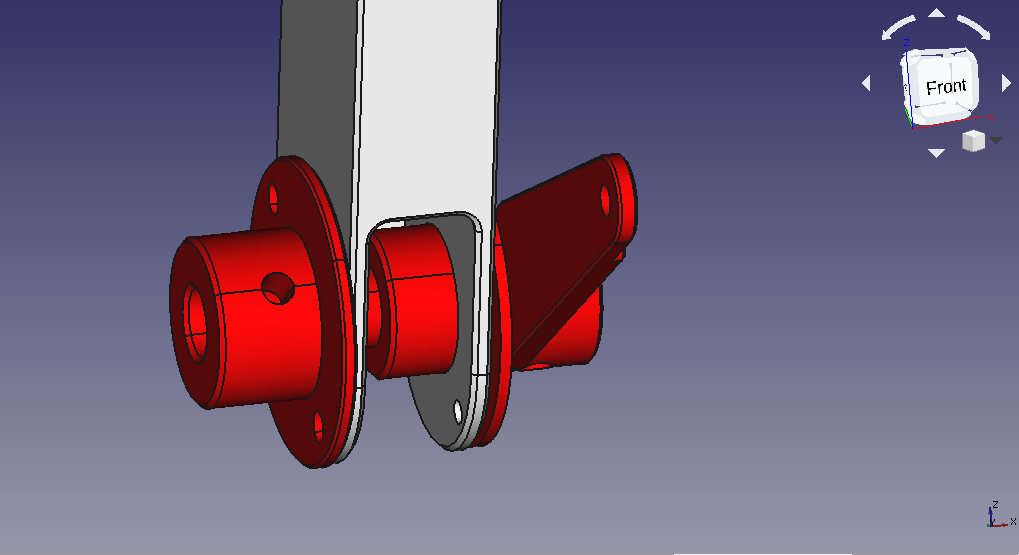
\includegraphics[width=1\linewidth]{pictures/SoporteMotorDerecho.png}
    \caption{Pieza derecha de la cadena de movimiento vertical}
    \label{fig:pieza_derecha_brazo}
\end{figure}

Finalmente se añade la pieza derecha según se observa en la figura \ref{fig:pieza_derecha_brazo}. Esta ultima es soportada por un eje metálico que atraviesa las 3 piezas.

En la parte superior del segmento central se monta una pieza según se observa en la figura \ref{fig:pieza_forma_rara}

\begin{figure}[H]
    \centering 
    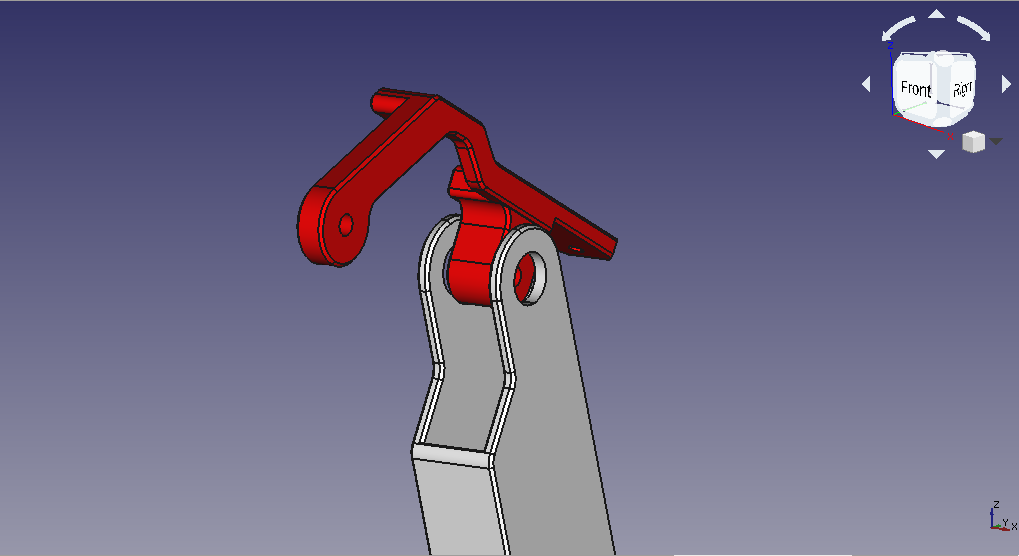
\includegraphics[width=1\linewidth]{pictures/PiezaConFormaRara.png}
    \caption{Pieza que sirve para unir el segmento inferior con el superior}
    \label{fig:pieza_forma_rara}
\end{figure}

Esta pieza se moverá de manera libre sobre un tornillo 4x15 mm que la atraviesa a modo de eje y que apoya sobre el segmento inferior en dos rodamientos los cuales se encuentran el las ranuras circulares que se observan en la figura \ref{fig:pieza_forma_rara}

Empleando esta pieza es posible asegurar el antebrazo en posición según se ve en la figura \ref{fig:antebrazo}. También se pueden apreciar los rodamientos de los que se hablaba en el párrafo anterior.

\begin{figure}[H]
    \centering 
    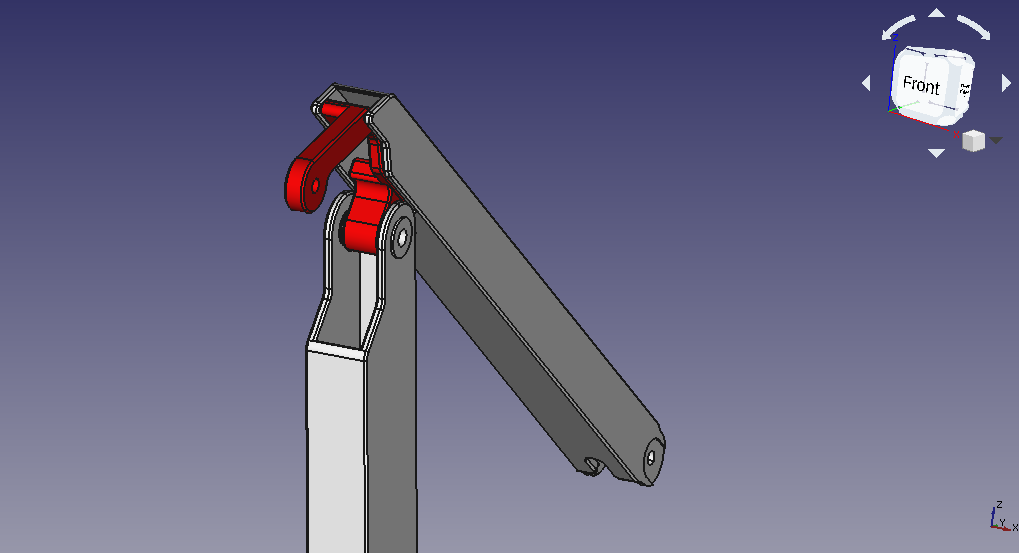
\includegraphics[width=1\linewidth]{pictures/Antebrazo.png}
    \caption{Antebrazo montado en la cadena articulada principal}
    \label{fig:antebrazo}
\end{figure}

Finalmente se añade a la cadena articulada principal el soporte del \textit{end--effector} según se observa en la figura \ref{fig:soporte_endeffector}. Este se mantiene unido al antebrazo mediante un tornillo de 4x15 mm el cual sirve de eje libre que lo atraviesa y se apoya en los dos rodamientos que se observan de color naranja en la figura.

\begin{figure}[H]
    \centering 
    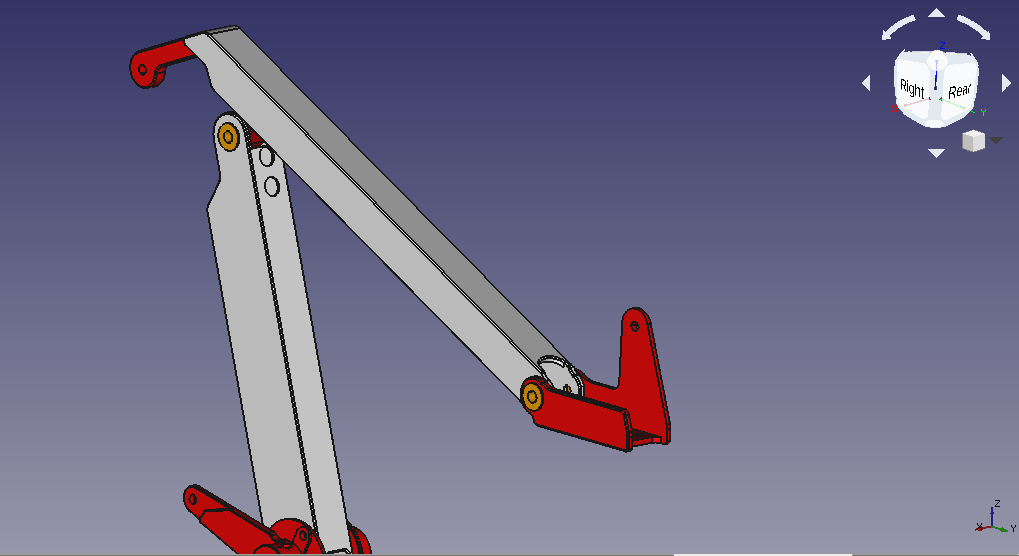
\includegraphics[width=1\linewidth]{pictures/SoporteEndEffector.png}
    \caption{Soporte del \textit{end--ffector}}
    \label{fig:soporte_endeffector}
\end{figure}

También se añade al soporte del \textit{end--efector} la sujeción para un posible motor que podría operar una pinza. Esto se puede ver en \ref{fig:soporte_motor}. Para asegurar esta pieza sobre el soporte, se emplean tornillos de 3x6 mm.

\begin{figure}[H]
    \centering 
    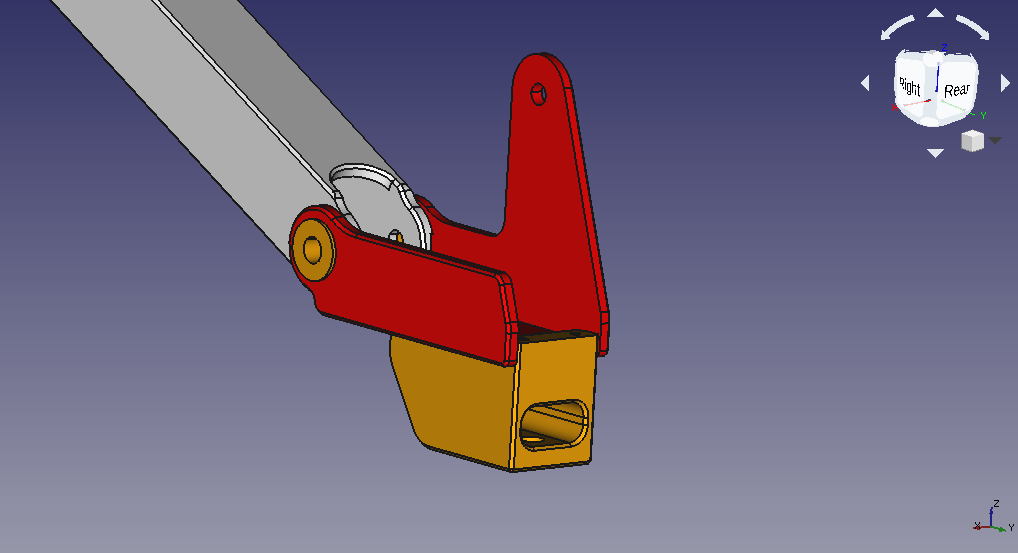
\includegraphics[width=1\linewidth]{pictures/SujecionMotorFinal.png}
    \caption{Soporte del motor que actúa sobre el \textit{end--effector}}
    \label{fig:soporte_motor}
\end{figure}

Llegados a este punto es preciso ensamblar las cadenas articuladas auxiliares las cuales permiten transmitir movimientos al antebrazo y al \textit{end--efector}.

Primero se ensambla la cadena auxiliar derecha según se observa en la figura \ref{fig:auxiliar_derecha}

\begin{figure}[H]
    \centering 
    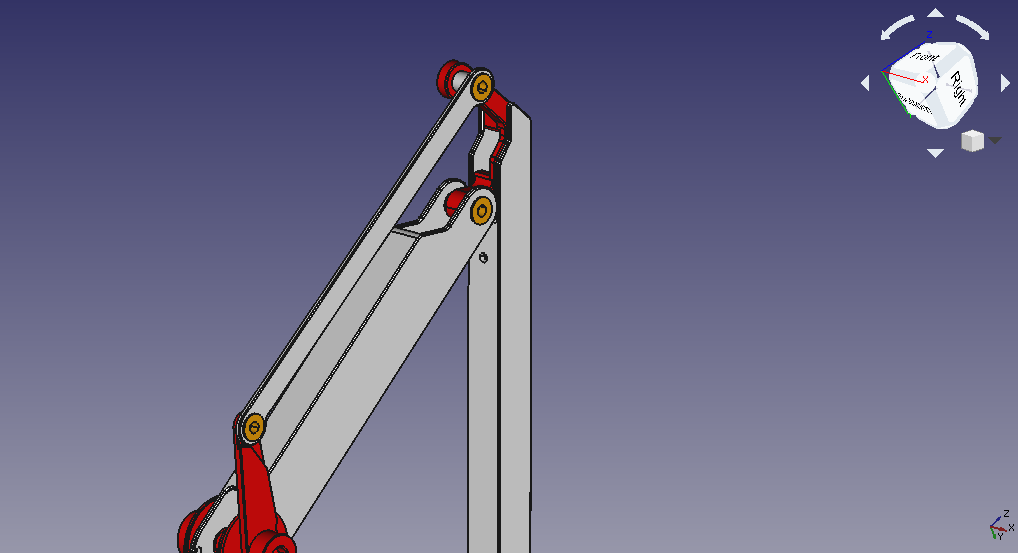
\includegraphics[width=1\linewidth]{pictures/CadenaArticuladaDerecha.png}
    \caption{Cadena articulada auxiliar derecha}
    \label{fig:auxiliar_derecha}
\end{figure}

La cadena auxiliar derecha se compone de una sola varilla que se ensambla en una de las piezas de la cadena de movimiento vertical, en la parte inferior del brazo, mediante un tornillo de 4x10 mm. En la parte superior la varilla se ensambla en la junta de unión del brazo con el antebrazo mediante un tornillo de 4x15 mm. Se puede observar que en ambos casos para permitir que los tornillos actúen como eje libre, estos se apoyan sobre rodamientos.

En segundo lugar se ensambla la cadena auxiliar izquierda. Se empieza añadiendo el triangulo de unión de las dos varillas que se explicarán mas adelante. Este triangulo se observa en la figura \ref{fig:triangulo_union_varillas}

\begin{figure}[H]
    \centering 
    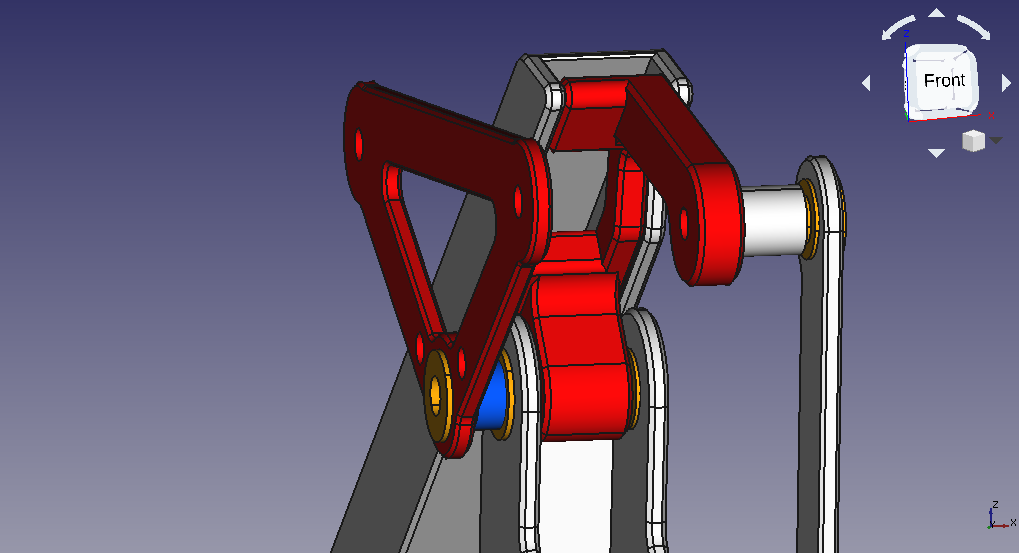
\includegraphics[width=1\linewidth]{pictures/TrianguloDeUnion.png}
    \caption{Triangulo de unión del las varillas de la cadena auxiliar izquierda}
    \label{fig:triangulo_union_varillas}
\end{figure}

Este triangulo se sujeta sobre el mismo eje que la junta de unión.
Se observa en azul un separador y en naranja el rodamiento gracias al cual se consigue que el tornillo sirva como eje libre.

Sobre este triangulo se añade una primera varilla que une el triangulo con uno de los soportes de los motores de la base, esta varilla se observa en la figura \ref{fig:varilla_inferior_izquierda}

\begin{figure}[H]
    \centering 
    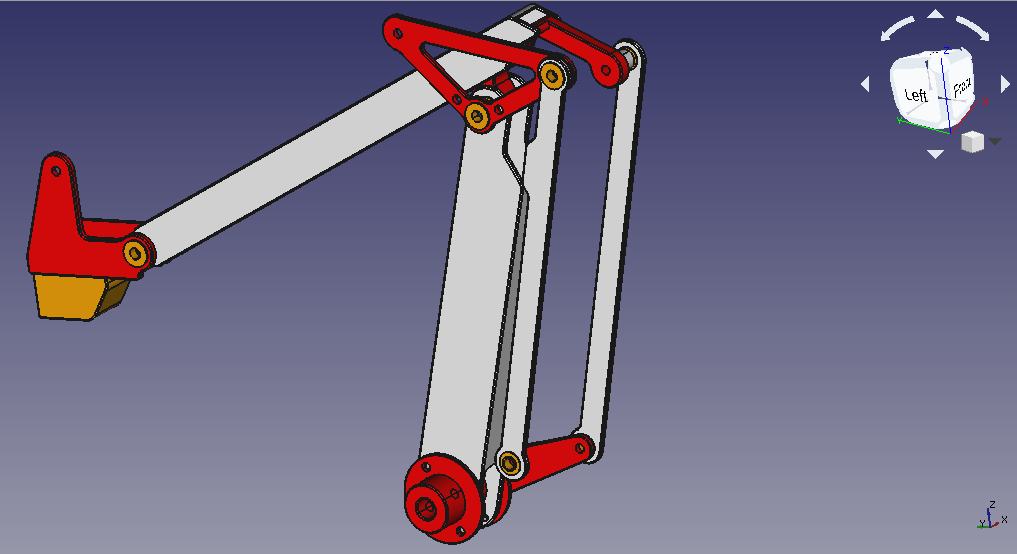
\includegraphics[width=1\linewidth]{pictures/VarillaInferior.png}
    \caption{Varilla inferior de la cadena auxiliar izquierda}
    \label{fig:varilla_inferior_izquierda}
\end{figure}

Esta varilla se sujeta en el triangulo mediante un tornillo de 4x10 mm el cual apoya sobre un rodamiento que hace que sirva de eje libre. En el soporte inferior del motor se sujeta mediante un tornillo de 4x40 mm.

Finalmente se une la varilla superior con el \textit{end--efector} mediante un tornillo de 4x10 mm y un rodamiento. En el triangulo se emplea el mismo método de sujeción. Esto se puede observar en la imagen \ref{fig:varilla_superior_izquierda}

\begin{figure}[H]
    \centering 
    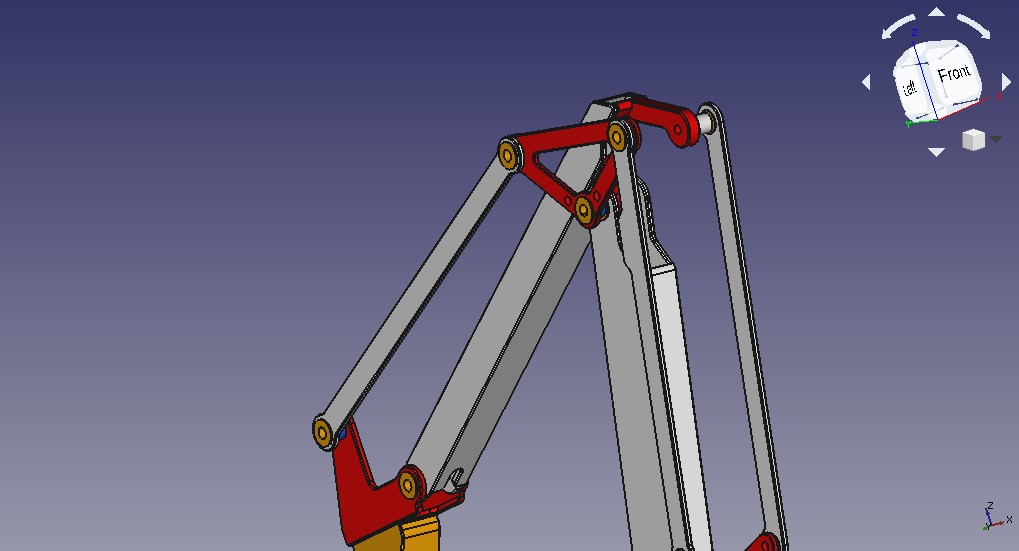
\includegraphics[width=1\linewidth]{pictures/VarillaSuperior.png}
    \caption{Varilla superior de la cadena auxiliar izquierda}
    \label{fig:varilla_superior_izquierda}
\end{figure}

Con esto finalizamos la construcción de la parte superior del brazo robótico y ya es posible introducirlo en la base rotatoria.

\begin{figure}[H]
    \centering 
    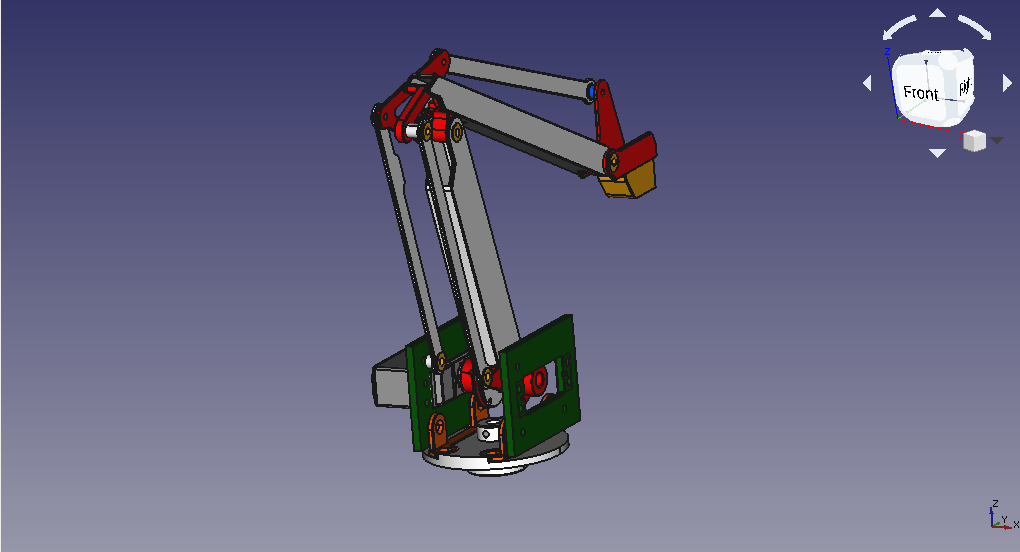
\includegraphics[width=1\linewidth]{pictures/ParteSuperiorDelBrazoEnElSoporte.png}
    \caption{La parte superior el brazo robótico ensamblada en la base rotativa.}
    \label{fig:parte_superio_ensamblada_base}
\end{figure}

Finalmente se coloca el ultimo motor y se deja la parte superior del brazo fijada entre los dos 




